\chapter{Marco teórico}
\label{ch:marco}

En este capítulo se presentan los conceptos en los que se basa el sistema propuesto para la solución de operaciones trigonométricas, en el formato de representación estándar de números en coma flotante, IEEE 754-2008, en concreto las operaciones seno y coseno. A continuación se brinda información acerca del formato de palabra para la representación binaria de números en punto flotante, ya sea en precisión simple o precisión doble, 32 y 64 bits respectivamente, así como para el manejo de la excepción de resultados \textit{Not a Number, NaN}.

Se presenta además las bases teóricas de la rotación de vectores, fundamento teórico en el que se sustenta el algoritmo CORDIC, investigado e implementado para la resolución de las operaciones trigonométricas antes mencionadas.


\section{Estándar IEEE 754}

El estándar IEEE 754 especifica formatos y métodos para aritmética en punto flotante en sistemas computacionales, permitiendo obtener el mismo resultado, dado el mismo dato de entrada, sin importar si el proceso es llevado a cabo en hardware, software, o una combinación de ambos \cite{IEEE754}. Para lograr esto, los diseñadores del estándar utilizaron el método de notación científica, permitiendo representar un número factorizándolo en dos partes, la magnitud y la potencia \cite{IEEE754_WEB}.

Los formatos de representación de números en punto flotante del estándar, son usados para representar un subconjunto finito de los números reales. Los formatos se caracterizan por: su base (binaria, decimal), precisión (simple, doble, extendida) y por el rango de su exponente, y cada uno puede representar un conjunto único de datos en punto flotante \cite{IEEE754}.

El estándar define 5 formatos básicos:

\begin{itemize}
	\item[-]	Tres formatos binarios, con codificaciones en longitud de 32, 64 y 128 bits.
	\item[-]	Dos formatos binarios, con codificaciones en longitud de 64 y 128 bits.
\end{itemize}

Las representaciones de un dato en punto flotante en un formato consiste en:

\begin{itemize}
	\item[-]	Triples (signo, exponente y significando); en una base b, el numero en punto flotante representado por un tripe tiene la siguiente forma:
    \begin{center} $(-1)^{signo} \times b^{exponente} \times significando $ \end{center}
	\item[-]	$+\infty, -\infty $
	\item[-]	$qNaN, sNaN$
\end{itemize}

El conjunto finito de números en punto flotante representables dentro de un formato en particular es determinado por determinados parámetros enteros, los cuales son: 

\begin{itemize}
	\item[-]		b = la base, 2 (binaria) o 10 (decimal).
	\item[-]		p = el número de dígitos en el significando, es decir, a precisión.
	\item[-]		\textit{emax} = el máximo exponente.
	\item[-]		\textit{emin} = el mínimo exponente.
\end{itemize}

Donde \textit{emin} = 1 - \textit{emax} para cada uno de los formatos.

En la Tabla \ref{Tabla_Parametros}  se presentan los valores de cada uno de los parámetros para cada uno de los formatos básicos, en el cuál cada formato está identificado por su base y el número de bits de su codificación.

\begin{table}[H]
\centering
\caption{Valores de los parámetros que definen los formatos básicos de números en punto flotante.7}
\label{Tabla_Parametros}
\begin{tabular}{c|c|c|c|c|c|}
\cline{2-6}
                                    & \multicolumn{3}{c|}{Formato Binario (b=2)}              & \multicolumn{2}{c|}{Formato Decimal (b=10)} \\ \hline
\multicolumn{1}{|c|}{parametro}     & binario(32 bits) & binario(64 bits) & binario(128 bits) & decimal64           & decimal 128           \\ \hline
\multicolumn{1}{|c|}{p, digitos}    & 24               & 53               & 113               & 16                  & 34                    \\ \hline
\multicolumn{1}{|c|}{\textit{emax}} & +127             & +1023            & +16383            & +384                & +6144                 \\ \hline
\end{tabular}
\end{table}

Sin importar el formato escogido, los siguientes datos deberán poder ser representados:

\begin{itemize}
	\item[-]	Cualquier número en punto flotante igual o diferente a cero y con signo de la forma:
	\begin{center} $(-1)^{s} \times b^{e} \times m $ \end{center}, donde
	\begin{itemize}
		\item	\textit{s} es igual a 1 o 0, donde 1 representa a los números negativos y el 0 a los números positivos.
		\item	\textit{e} corresponde a cualquier numero entero entre $emin \leq e \leq emax$.
		\item	\textit{m} es un número representado por una cadena de dígitos de la forma $ d0*d1d2...d_{p-1} $, donde $ d_{i} $ es un dígito entero entre $ 0 \leq di \leq b $, por lo tanto \textit{m} puede ser un valor  entre $ 0 \leq m \leq b $.
		
	\end{itemize}
	\item[-]	Dos valores infinitos, $ +\infty,-\infty $.
	\item[-]	Dos representaciones \textit{NaN}, \textit{qNaN} y \textit{sNaN}.
\end{itemize}

El número positivo más pequeño representable en cada formato es $b^{emin}$, mientras que el más grande es $b^{emax}*(b-b^{1-p})$. Los números diferentes a cero con magnitudes menores a $b^{emin}$ son llamados subnormales, debido a que sus magnitudes caen en valores entre cero y el número normal más pequeño.

En la notación científica, los números pueden tener exponentes tanto negativos como positivos. En la representación binaria, el exponente debe ser  normalizado para ser utilizado, ya que en un sistema computacional un exponente negativo debería ser almacenado utilizando una representación en complemento a 2, pero para fines de comparación entre valores, la comparación de valores en complemento a 2 es más compleja que comparar valores que no posean signo, por lo que al exponente se le suma un valor de sesgo para normalizar dicho exponente, para ubicarlo dentro de los valores positivos siempre. Este valor de sesgo tiene un valor igual a \textit{emin}, por lo que el valor del exponente normalizado vendría dado por (\ref{eq:Ec_esp_norm})  \cite{Tesis_Diego}.

\begin{equation}\label{eq:Ec_esp_norm}
Exponente\_normalizado = Exponente - emin
\end{equation}

\subsection{Formatos de precisión en punto flotante.}

Como se menciona anteriormente, en el estándar IEEE 754 existen varios formatos de representación de números en punto flotante, ya sean binarios, decimales o formatos extendidos.

Los formatos de precisión, o almacenamiento, determinan la cantidad de espacio en memoria que un valor en punto flotante necesita en memoria para ser almacenado, y son utilizados para representar un subconjunto definido finito de números reales. Cada formato se diferencia de los demás por la ubicación del punto decimal, la precisión del dato y el rango de su exponente, así como el hecho de que cada uno puede representar solo un determinado conjunto de números en punto flotante \cite{Tesis_Diego}.

Los formatos que se desarrollan en este documento tienen una distribución definida de bits, para representar un valor en punto flotante. En la Figura \ref{fig:acomodo_bits} se observa el acomodo de los diferentes campos que conforman la representación según el estándar IEEE 754 \cite{IEEE754}.


\begin{figure}[htb]
  \centering
  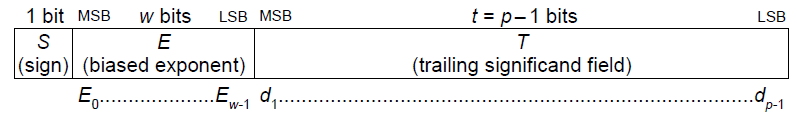
\includegraphics[width=0.7\textwidth]{acomodo_bits}
  \caption{Acomodo de bits para la representación binaria de un número en punto flotante utilizando el estándar IEEE 754-2008.}
  \label{fig:acomodo_bits}
\end{figure}


En este documento solo se tratan dos formatos de precisión binarios, el formato de precisión simple y el de precisión doble, y al igual que los formatos decimales y extendidos, se caracterizan por tener un ancho de palabra definido.

Según el patrón de bits presente en la representación binaria de un número en punto flotante, así será su interpretación. En la Tabla \ref{int_patron} se presenta la interpretación de dichos patrones según los valores en los campos de la representación, ya sea para precisión simple o doble \cite{Tesis_Diego}.



\begin{table}[htb]
\centering
\caption{Interpretación de patrones de bits del estándar IEEE 754 para el formato de precisión simple y doble.}
\label{int_patron}
\begin{tabular}{c|c|c|}
\cline{2-3}
                                                                                                                              & \multicolumn{2}{c|}{Patrón de bits}                                                                                                                                                                                                                                                               \\ \hline
\multicolumn{1}{|c|}{\begin{tabular}[c]{@{}c@{}}Tipo de\\  Número\end{tabular}}                                               & Precisión Simple                                                                                                                                & Precisión Doble                                                                                                                                 \\ \hline
\multicolumn{1}{|c|}{\begin{tabular}[c]{@{}c@{}}Números \\ Normales\end{tabular}}                                             & \begin{tabular}[c]{@{}c@{}}Signo = 0 ó 1\\ $00_{h}<$Exponente Normalizado $< ff_{h}$\\ Fracción = Cualquier combinación \\ de bits\end{tabular} & \begin{tabular}[c]{@{}c@{}}Signo = 0 ó 1\\ $000_{h}<$Exponente Normalizado$<7ff_{h}$\\ Fracción = Cualquier combinación\\  de bits\end{tabular} \\ \hline
\multicolumn{1}{|c|}{\begin{tabular}[c]{@{}c@{}}Números \\ Subnormales\end{tabular}}                                          & \begin{tabular}[c]{@{}c@{}}Signo = 0 ó 1 \\ Exponente Normalizado = $00_{h}$ \\  Fracción $\neq 00000_{h}$\end{tabular}                         & \begin{tabular}[c]{@{}c@{}}Signo = 0 ó 1\\ Exponente Normalizado = $000_{h}$\\ Fracción $\neq 0000000000000_{h}$\end{tabular}                   \\ \hline
\multicolumn{1}{|c|}{\begin{tabular}[c]{@{}c@{}}Caso Especial \\  Cero con Signo\end{tabular}}                                & \begin{tabular}[c]{@{}c@{}}Signo = 0 ó 1 \\ Exponente Normalizado = $00_{h}$\\ Fracción $= 000000_{h}$\end{tabular}                             & \begin{tabular}[c]{@{}c@{}}Signo = 0 ó 1\\ Exponente Normalizado = $000_{h}$\\ Fracción $=0000000000000_{h}$\end{tabular}                       \\ \hline
\multicolumn{1}{|c|}{\begin{tabular}[c]{@{}c@{}}Caso Especial \\ Infinito Positivo\end{tabular}}                              & \begin{tabular}[c]{@{}c@{}}Signo = 0\\ Exponente Normalizado = $ff_{h}$\\ Fracción $= 00_{h}$\end{tabular}                                      & \begin{tabular}[c]{@{}c@{}}Signo = 0\\ Exponente Normalizado = $7ff_{h}$\\ Fracción $= 0000000000000_{h}$\end{tabular}                          \\ \hline
\multicolumn{1}{|c|}{\begin{tabular}[c]{@{}c@{}}Caso Especial\\ Infinito Negativo\end{tabular}}                               & \begin{tabular}[c]{@{}c@{}}Signo = 1\\ Exponente Normalizado = $ff_{h}$\\ Fracción $= 00_{h}$\end{tabular}                                      & \begin{tabular}[c]{@{}c@{}}Signo = 1\\ Exponente Normalizado = $7ff_{h}$\\ Fracción $= 000000000000_{h}$\end{tabular}                           \\ \hline
\multicolumn{1}{|c|}{\begin{tabular}[c]{@{}c@{}}Caso Especial\\  Números no\\  representables \\ (Not a Number)\end{tabular}} & \begin{tabular}[c]{@{}c@{}}Signo = 0 ó 1\\ Exponente Normalizado = $ff_{h}$\\  Fracción $\neq 00000_{h}$\end{tabular}                           & \begin{tabular}[c]{@{}c@{}}Signo = 0 ó 1\\ Exponente Normalizado = $7ff_{h}$ \\ Fracción $\neq 000000000000_{h}$\end{tabular}                   \\ \hline
\end{tabular}
\end{table}


\subsubsection{Formato de Precisión Simple.}

Este formato de precisión tiene un ancho de palabra definido de 32 bits, de los cuales el campo de signo ocupa 1 bit, el bit más significativo de la cadena de bits, y puede tomar dos valores únicamente, 0 que representa a los números positivos, y 1 que representa a los números negativos. El campo de exponente ocupa los 8 bits después del bit de signo, siguiendo la dirección del MSB al LSB, por lo que el exponente puede tomar cualquier valor desde 0 a 255, donde los valores desde 0 a 127 representan los exponentes negativos, y desde 128 a 255 representan los exponentes positivos. Por último, el campo de mantisa ocupa 23 bits.

En la Figura \ref{fig:dist_form_sim} se muestra la distribución de bits de cada campo para el formato de precisión simple.

\begin{figure}[htb]
  \centering
  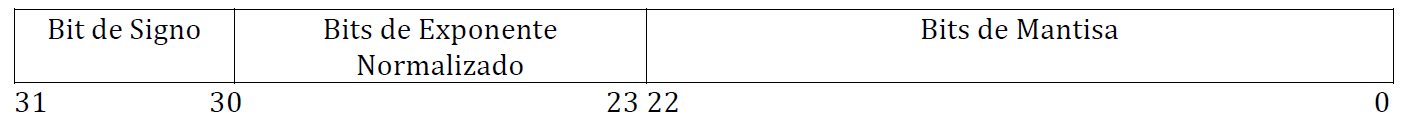
\includegraphics[width=0.7\textwidth]{dist_form_sim}
  \caption{Ordenamiento de bits en el formato de Precisión Simple.}
  \label{fig:dist_form_sim}
\end{figure}

La normalización del exponente para este formato se lleva a cabo con un valor de sesgo de 127.

\subsubsection{Formato de Precisión Doble.}

En el formato de precisión doble se tiene un ancho de palabra definido de 64 bits, de los cuales el campo de signo, al igual que en el formato de precisión simple, ocupa 1 bit, el bit más significativo de la cadena de bits, y puede tomar dos valores únicamente, 0 que representa a los números positivos, y 1 que representa a los números negativos. El campo de exponente ocupa los once bits después del bit de signo, siguiendo la dirección del MSB al LSB.. Por último, el campo de mantisa ocupa 52 bits.

En la Figura \ref{fig:dist_form_dob} se muestra la distribución de bits de cada campo para el formato de precisión doble.

\begin{figure}[htb]
  \centering
  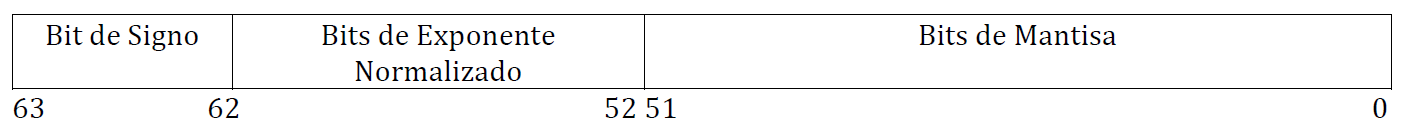
\includegraphics[width=0.7\textwidth]{dist_form_dob}
  \caption{Ordenamiento de bits en el formato de Precisión Doble.}
  \label{fig:dist_form_dob}
\end{figure}

La normalización del exponente para este formato se lleva a cabo con un valor de sesgo de 1023.

\section{Algoritmo CORDIC para el cálculo de operaciones trigonométricas.}

El algoritmo de Computación Digital para Rotación de Coordenadas, CORDIC por sus siglas en inglés (\textbf{CO}ordinate \textbf{R}otation \textbf{D}igital \textbf{C}omputer), fue desarrollado especialmente para usarse en computadoras digitales en tiempo real, donde la mayoría de la computación involucraba la resolución de las relaciones trigonométricas de las ecuaciones de navegación y una alta tasa de exactitud para las relaciones trigonométricas de las transformaciones de coordenadas \cite{CORDIC}.

Este algoritmo fue  originalmente propuesto por Jack Volder en el año 1959, con el propósito de calcular funciones trigonométricas mediante la rotación de vectores. La rotación de vectores es usada también para realizar la conversión de sistemas coordenados (polar a cartesiano y viceversa), y como parte de funciones matemáticas más complejas como lo son la Transformada Rápida de Fourier (FFT), y la transformada Coseno Discreta (DCT).

El CORDIC es un algoritmo iterativo para rotar vectores a ciertos ángulos determinados, que efectúa operaciones matemáticas a alta velocidad en sistemas coordenados lineales, circulares e hiperbólicos y que solo utiliza operaciones de suma y desplazamiento para efectuar operaciones trigonométricas, exponenciales, logarítmicas, y otras funciones trascendentales \cite{DoubleCordic}.


\subsection{Fundamento Teórico.}

El algoritmo originalmente propuesto \cite{CORDIC}, describe la rotación de un vector bidimensional en el plano cartesiano, como el mostrado en la Figura \ref{fig:rot_vector}. El funcionamiento del algoritmo se deduce de la formula general de rotación de vectores:

\begin{equation}\label{eq:ec_rot_vectores}
\begin{array}{l}
     x^{\prime} = xcos \theta - ysen \theta \\
     y^{\prime} = ycos \theta + xsen \theta \\
\end{array}
\end{equation}

\begin{figure}[htb]
  \centering
  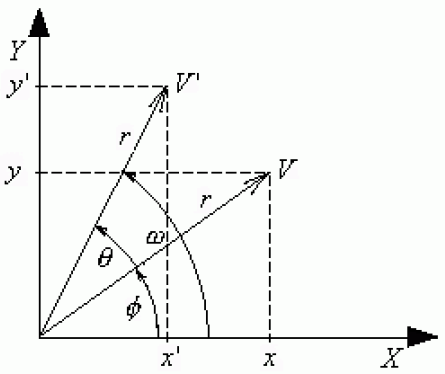
\includegraphics[width=0.3\textwidth]{rot_vector}
  \caption{Vector bidimensional antes y después de ser rotado.}
  \label{fig:rot_vector}
\end{figure}

Sacando a factor común el $cos\theta$ en la Ecuación (\ref{eq:ec_rot_vectores}), asumiendo que $cos\theta \neq 0$, se obtiene

\begin{equation}\label{eq:ec_rot_vectores2}
\begin{array}{l}
     x^{\prime} = cos \theta(x - ytan \theta )\\
     y^{\prime} = cos \theta(y + xtan \theta )\\
\end{array}
\end{equation}

Y tomando en cuenta que,

\begin{equation}\label{eq:cos_cita}
 cos\theta = \dfrac{1}{\sqrt{1 + tan^{2}\theta}}
\end{equation}

Entonces la Ecuación (\ref{eq:ec_rot_vectores2}) se puede expresar como

\begin{equation}\label{eq:ec_rot_vectores3}
\begin{array}{l}
     x^{\prime} = \dfrac{x-ytan\theta}{\sqrt{1 + tan^{2}\theta}}\\
     y^{\prime} = \dfrac{y+xtan\theta}{\sqrt{1 + tan^{2}\theta}}\\
\end{array}
\end{equation}

En el algoritmo CORDIC, las rotaciones son substituidas por pseudorotaciones vectoriales, tal y como se muestra en la Figura \ref{fig:pseudorotacion}.

\begin{figure}[htb]
  \centering
  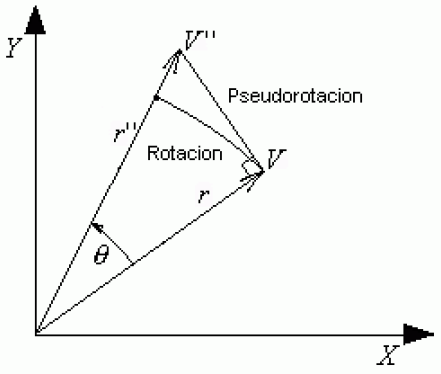
\includegraphics[width=0.3\textwidth]{pseudorotacion}
  \caption{Pseudorotación de un vector bidimensional.}
  \label{fig:pseudorotacion}
\end{figure}

En una rotación real no se cambia la magnitud del vector V una vez realizada la rotación, pero en una pseudorotación esto no aplica, ya que incrementa su magnitud en

\begin{equation} \label{eq:mag_pseudo}
V^{\prime \prime} = V\sqrt{1 + tan^{2}\theta}
\end{equation}

La rotación de un ángulo se puede descomponer en una sumatoria de rotaciones más pequeñas. Asumiendo inicialmente que $x=x_{0}$,  $y=y_{0}$ y $z=z_{0}$, después de realizadas n iteraciones para una rotación real, se obtiene


\begin{equation}\label{eq:ec_rot_real_x}
     x^{\prime}_{n} = xcos\theta(\sum_{i=0}^{n-1}\theta_{i}) - ysin\theta(\sum_{i=0}^{n-1}\theta_{i})
\end{equation}

\begin{equation}\label{eq:ec_rot_real_y}
     y^{\prime}_{n} = ycos\theta(\sum_{i=0}^{n-1}\theta_{i}) + xsin\theta(\sum_{i=0}^{n-1}\theta_{i})
\end{equation}

\begin{equation}\label{eq:ec_rot_real_z}
	z^{\prime}_{n} = z - (\sum_{i=0}^{n-1}\theta_{i})\\
\end{equation}

En cambio para una pseudorotación se obtiene

\begin{equation}\label{eq:ec_rot_real_x1}
     x^{\prime\prime}_{n} = (xcos\theta(\sum_{i=0}^{n-1}\theta_{i}) - ysin\theta(\sum_{i=0}^{n-1}\theta_{i}))\prod_{i=0}^{n-1}\sqrt{1 + tan^{2}\theta_{i}}
\end{equation}

\begin{equation}\label{eq:ec_rot_real_y1}
     y^{\prime\prime}_{n} = (ycos\theta(\sum_{i=0}^{n-1}\theta_{i}) + xsin\theta(\sum_{i=0}^{n-1}\theta_{i}))\prod_{i=0}^{n-1}\sqrt{1 + tan^{2}\theta_{i}}
\end{equation}

\begin{equation}\label{eq:ec_rot_real_z1}
	z^{\prime\prime}_{n} = z - (\sum_{i=0}^{n-1}\theta_{i})\\
\end{equation}

, en donde \[\sum_{i=0}^{n-1}\theta_{i} = \theta\]

Las Ecuaciones (\ref{eq:ec_rot_real_z}) y (\ref{eq:ec_rot_real_z1}) son conocidas como el parámetro \textit{acumulador angular}, ya que incluye las rotaciones realizadas hasta el momento.

Si se restringen los ángulos de rotación de tal manera que $tan\theta = \pm2^{-i}, i\in N$, la operación multiplicación, que es tan costosa para un sistema computacional en términos de área y  tiempo, se ve reducida a una operación de desplazamiento. Además, los diversos ángulos se pueden obtener al realizar una sucesión de rotaciones elementales cada vez mas pequeñas, y en cada iteración, en vez de de determinar si se debe rotar o no, lo que hace es escoger el sentido de rotación.

Tomando como punto de partida las Ecuaciones (\ref{eq:ec_rot_vectores2}),sustituyendo $tan\theta = \pm2^{-i}$,y además teniendo en cuenta que $cos(\theta) =  cos(-\theta)$,las iteraciones se pueden expresar como


\begin{equation}\label{eq:ec_rot_vectores_4}
\begin{array}{l}
     x_{i+1} = K_{i}(x_{i} - y_{i}d_{i}2^{-i})\\
     y_{i+1} = K_{i}(y_{i} + x_{i}d_{i}2^{-i})\\
\end{array}
\end{equation}

en donde $K_{i}=\dfrac{1}{\sqrt{1+2^{-2i}}}$ y $d_{i} = \pm 1 $ dependiendo del sentido de rotación.

Esta valor $K_{i}$, debe ser multiplicado por las ecuaciones correspondientes a las pseudorotaciones, para obtener la rotación real, ya que como se menciono anteriormente, las pseudorotaciones aumentan el tamaño del vector, por lo que el valor $K_{i}$ contrarrestaría este efecto.

Eliminando el valor $K_{i}$ de las ecuaciones iterativas, se obtiene un algoritmo basado en sumas y desplazamientos, y factor $K_{i}$ puede aplicarse al final o al principio del proceso como una constante $K_{n}$, definida como

\begin{equation}\label{eq:Kn}
K_{n}=\lim_{n  \rightarrow \infty}\prod_{i=0}^{n}K_{i}\cong 0.607253
\end{equation}
 
El valor exacto de la constante $K_{n}$ es determinado por la cantidad de iteraciones realizadas.

En cada paso de iteración, el algoritmo, en vez de decidir si se rota o no, lo que decide es el signo o sentido de rotación que se efectuara. por esto mismo, cada ángulo final se puede representar mediante un vector de signos, en donde cada componente corresponde a un ángulo de la secuencia de ángulos elementales. Estos ángulos se almacenan en una Look-Up Table(LUT). Dependiendo del sistema angular, se almacenan en la tabla las arcotangentes correspondientes a ese sistema.  Con esta último punto, se puede modificar el acumulador angular, obteniendo

\begin{equation}\label{eq:acum_fin}
z_{i+1}=z_{i}-d_{i}arctan(2^{-i})
\end{equation}

El algoritmo CORDIC puede trabajar u operar en dos modos, \textit{rotación}(rotation) o \textit{vectorización}(vectoring). En primero rota el vector de entrada un ángulo específico que se introduce como parámetro. El segundo modo rota el vector de entrada hacia el eje \textit{X}, acumulando el ángulo necesario para efectuar dicha rotación.

En el caso del modo de \textit{rotación}, el acumulador angular es inicializado con el ángulo a rotar, y la decisión sobre el sentido de rotación en cada iteración, se realiza para minimizar la magnitud del ángulo acumulado, hasta llegar a cero, con lo que el signo que determina el sentido de rotación, se obtiene del valor del acumulador angular en cada iteración.

Para el modo de \textit{rotación}, las ecuaciones iterativas son

\begin{equation}\label{eq:ec_rotacion}
\begin{array}{l}
     x_{i+1} = x_{i} - y_{i}d_{i}2^{-i}\\
     y_{i+1} = y_{i} + x_{i}d_{i}2^{-i}\\
     z_{i+1} = z_{i} - d_{i}arctan(2^{-i})\\
\end{array}
\end{equation}

en donde, $d_{i}$ = $\left\lbrace
\begin{array}{l}
     -1 ,z_{i} < 0\\
     +1 ,z_{i} \geqslant 0 \\
\end{array}
\right.$


Para el modo de \textit{vectorización}, el ángulo que ingresa se rota hasta quedar alineado con el eje \textit{X}. Este resultado se logra minimizando la magnitud del componente \textit{y}, en vez de la magnitud del acumulador angular. a diferencia del modo de \textit{rotación}, se utiliza el signo de la variable \textit{y} para definir la dirección de rotación de la siguiente iteración. Si se inicia el acumulador angular con el valor cero, al finalizar el proceso esta variable contendrá el ángulo de rotación adecuado.

Para el modo de \textit{vectorización}, las ecuaciones iterativas son

\begin{equation}\label{eq:ec_rotacion}
\begin{array}{l}
     x_{i+1} = x_{i} - y_{i}d_{i}2^{-i}\\
     y_{i+1} = y_{i} + x_{i}d_{i}2^{-i}\\
     z_{i+1} = z_{i} - d_{i}arctan(2^{-i})\\
\end{array}
\end{equation}

en donde, $d_{i}$ = $\left\lbrace
\begin{array}{l}
     -1 ,y_{i} \geqslant 0\\
     +1 ,y_{i} < 0 \\
\end{array}
\right.$

Cabe destacar que el algoritmo CORDIC está restringido a rango de ángulos $\dfrac{-\pi}{2} \leqslant \theta \leqslant \dfrac{\pi}{2}$, esto debido a que los ángulos elementales convergen sólo dentro de ester rango, y para tratar ángulos por fuera de ese rango, estos se deben de reducir al primer o cuarto cuadrante.

\section{Arquitecturas de implementación del algoritmo \textbf{CORDIC}.}

\subsection{Arquitectura Bit-Paralela Iterativa.}

La arquitectura bit-paralela es una las más utilizadas a la hora de implementar el algoritmo CORDIC en hardware. Se denomina paralela por la forma en que se opera con las componentes \textit{X, Y y Z}. Cada etapa de esta implementación consiste en un registro para almacenar los valores de salida, una unidad del desplazamiento y un sumador algebraico. 

Cuando se inicia el cálculo, los valores iniciales para $x_{0}, y_{0} y z_{0}$ ingresan de manera paralela a los registros a través de los multiplexores de 2x1. El bit más siginificativo de la variable \textit{X o Y}, dependiendo del modo, en cada paso iterativo determina la operación a efectuar por el sumador. Seguidamente, las señales de las variables \textit{X y Y} son desplazadas, y luego sumadas o restadas a las mismas señales sin desplazar, correspondiente a la variable opuesta. 

La variable \textit{Z} suma o resta los valores almacenados en el registro con los valores almacenados en una Look-Up Table, (\textit{LUT}), de arcotangentes precalculadas con una cantidad de entradas proporcional a la cantidad de iteraciones. Dicha \textit{LUT} puede ser implementada en una memoria ROM. Cuando se alcanza la iteración n, el valor a calcular se puede obtener en la salida. 

Esta arquitectura tiene como ventaja el uso eficiente de hardware, debido a que los recursos son reutilizados en cada iteración. En la Figura \ref{fig:bit_paralela} se muestra el diagrama correspondiente a la arquitectura antes descrita. A esta arquitectura además, se le debe implementar una maquina de control que controle el flujo de los datos, además de controlar las iteraciones realizas, el canal de mux a activar, entre otras cosas.

\begin{figure}[htb]
  \centering
  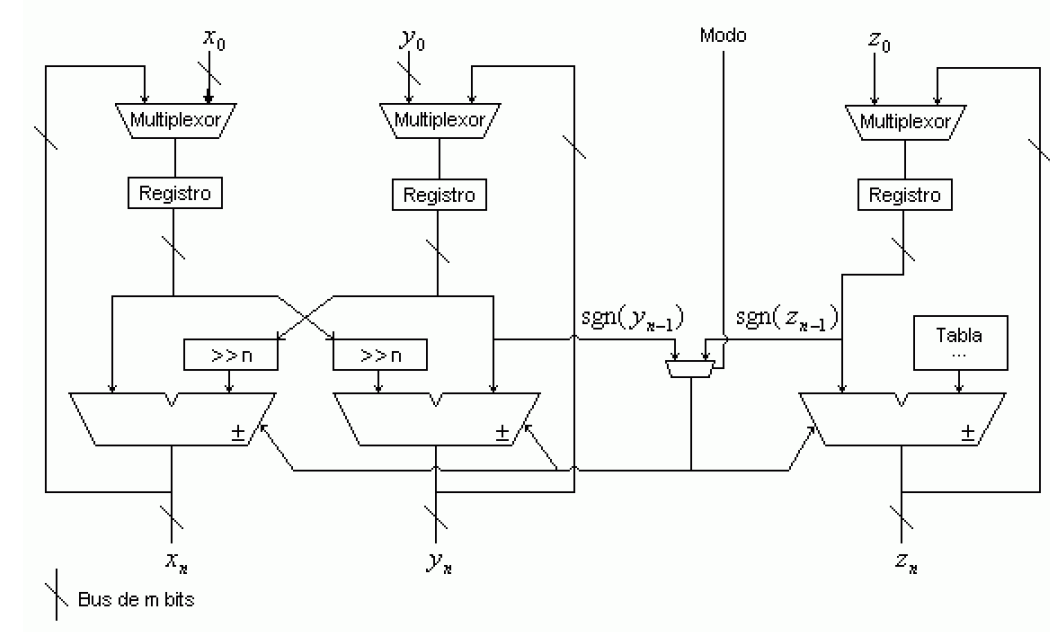
\includegraphics[width=0.7\textwidth]{bit_paralela}
  \caption{Arquitectura Bit-Paralela Iterativa para la implementación en hardware del algoritmo \textbf{CORDIC}.}
  \label{fig:bit_paralela}
\end{figure}

\subsection{Arquitectura Bit-Paralela Desplegada.}


Esta arquitectura, en vez de almacenar el resultado de cada iteración en registros y volver a utilizar los mismos recursos, tal como lo hacia la arquitectura anterior, despliega su diseño de manera que se separa en etapas correspondientes a cada iteración. Cada una de las etapas está compuesta por los mismos componentes, las dos unidades de desplazamiento y tres sumadores algebraicos, por lo que las salidas de una etapa corresponden a la entrada de la siguiente, y el diseño se vuelve completamente combinatorio.

El desarrollar el algoritmo CORDIC por medio de esta arquitectura provee dos ventajas: 
\begin{itemize}
\item[-]	Las unidades de desplazamiento y las constantes correspondientes a cada iteración pueden ser cableadas.
\item[-]	Al ser el diseño completamente combinatorio, no se requiere de una maquina de control, lo que simplifica bastante el diseño.
\end{itemize}

Pero, presenta una gran desventaja, debido a la gran cantidad de recursos de hardware que consume, ya que en este diseño se requiere replicar cada etapa n veces, igual a la cantidad de iteraciones que tomaria en la arquitectura bit-paralela iterativa, para conseguir un resultado similar.

En la Figura \ref{fig:bit_paralela2} se observa el esquema de la arquitectura Bit- Paralela Desplegada, donde se observa que cada componente presente en la arquitectura Bit-Paralela Iterativa, a excepción de los registros y de la \textit{LUT}, que es cambiada por constantes en cada sumador algebraico utilizado en el acumulador algebraico, la variable \textit{z}, se debe repetir \textit{n} veces.


\begin{figure}[htb]
  \centering
  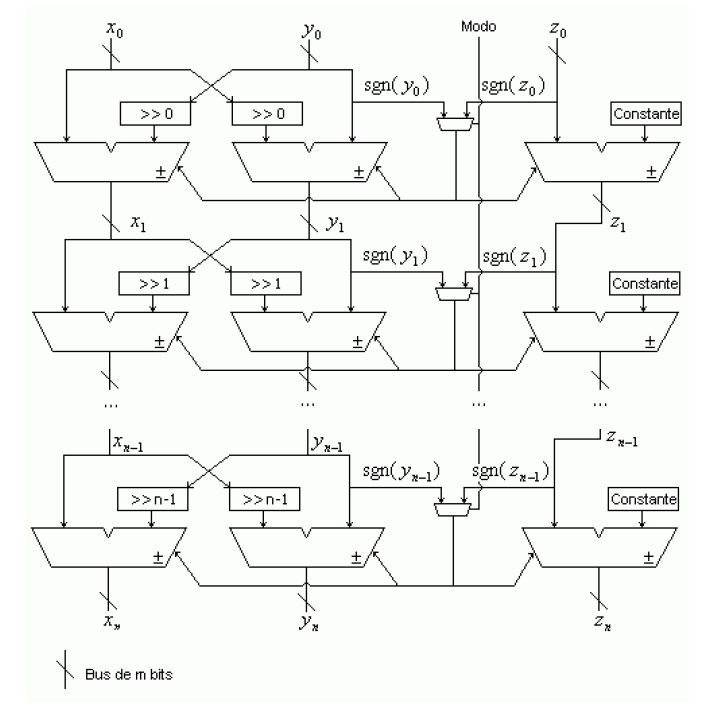
\includegraphics[width=0.7\textwidth]{bit_paralela2}
  \caption{Arquitectura Bit-Paralela Desplegada para la implementación en hardware del algoritmo \textbf{CORDIC}.}
  \label{fig:bit_paralela2}
\end{figure}

\subsection{Arquitectura Bit-Serie Iterativa.}


En esta arquitectura, se procesa un bit a la vez, con lo que las conexiones se reducen a un bit de ancho. En este diseño, cada etapa del algoritmo está conformada por tres multiplexores, dos registros de desplazamiento y 3 sumadores algebraico bit-serie. Estos sumadores se implementan como un sumador completo, en el que la resta se lleva a cabo sumando el complemento a dos del valor a restar.

El desempeño de esta arquitectura pude ser calculado como

\begin{equation}\label{eq:desem-serie}
\delta = \dfrac{f}{n \dot{•} W}
\end{equation}
,donde \textit{f} es la frecuencia de reloj del sistema, \textit{n} la cantidad de iteraciones a realizar y \textit{W} el ancho de palabra. En la Figura \ref{fig:bit_serie} se observa el esquema de esta arquitectura.

\begin{figure}[htb]
  \centering
  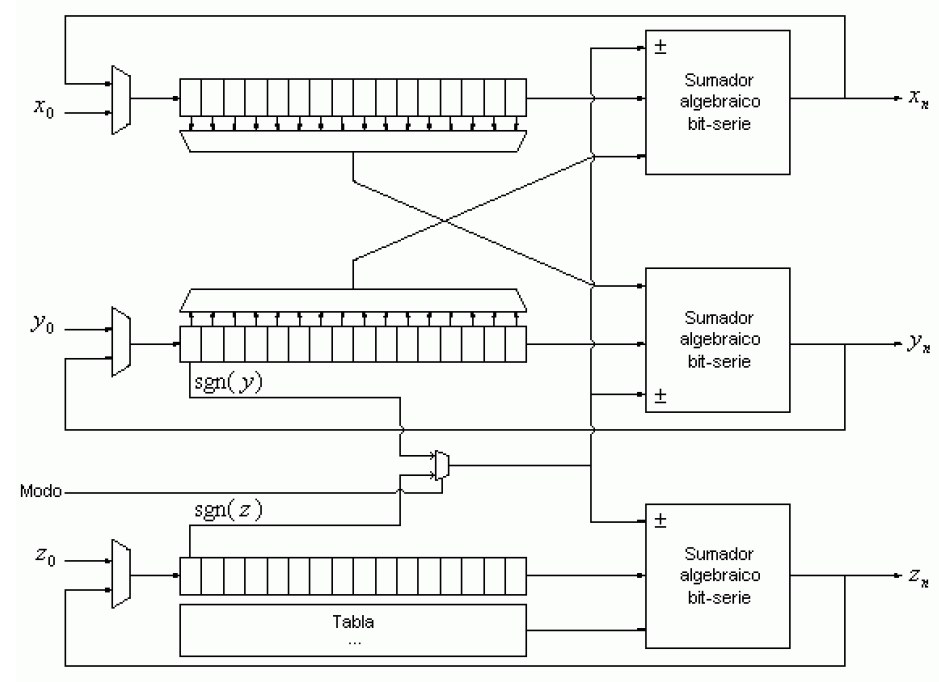
\includegraphics[width=0.7\textwidth]{bit_serie}
  \caption{Arquitectura Bit-Serie Iterativa para la implementación en hardware del algoritmo \textbf{CORDIC}.}
  \label{fig:bit_serie}
\end{figure}

La ventaja que presenta esta arquitectura es que los buses de interconexión son del ancho de un bit y que el registro de desplazamiento está integrado al registro intermedio que se utilizaba en la arquitectura Bit-Paralela Iterativa, lo que minimiza el espacio a la hora de la implementación, en comparación con dicha arquitectura. 

Pero por otro lado presenta dos grandes desventajas. Primero que introduce un retardo proporcional al ancho de palabra en cada etapa, esto ocasionado por los registros de desplazamiento, y segundo, es que esta arquitectura requeriría una maquina de control más compleja que la que se necesita en la arquitectura Bit-Paralela Iterativa.









%La Ecuación (\ref{eq:ec_rot_vectores}) es deducida a partir de las identidades trigonométricas básicas, donde

%\begin{equation}\label{eq:ec_trig_basic1}
%V : \left\lbrace
%\begin{array}{l}
%     x = rcos\phi \\
%     y = rsen\phi \\
%\end{array}
%\right.
%\end{equation}

%\begin{equation}\label{eq:ec_trig_basic2}
%V^{\prime} : \left\lbrace
%\begin{array}{l}
%     x^{\prime} = rcos\omega \\
%     y^{\prime} = rsen\omega \\
%\end{array}
%\right.
%\end{equation}

%Definiendo r=1 y $ \theta = \omega -\phi $, entonces $\omega = \theta +  \phi$. Con estas definiciones y utilizando las identidades de suma de  ángulos %para el seno y el coseno se obtiene


%\begin{equation}\label{eq:ec_sum_angulos}
%\begin{array}{l}
%     x^{\prime} = cos(\theta + \phi) = cos\theta cos\phi - sin\theta sin\phi = xcos\theta - ysin\theta\\
%     y^{\prime} = sin(\theta + \phi) = sin\theta cos\phi + cos\theta sin\phi = xsin\theta + ycos\theta\\
%\end{array}
%\end{equation}


\subsection{Ecuaciones}

%Para citar \nt{ecuaciones} se utilizan paréntesis redondos, y no es necesario
%emplear la palabra ``ecuación''. Por ejemplo ``Introduciendo en (4.2) los
%resultados de (3.3) y (3.7) se obtiene ...''. La ecuación es parte del flujo de
%texto y no un objeto flotante, así que no pueden emplearse como figuras. Cuando
%se requiere la ecuación, allí se inserta.  

%Es incorrecto redactar de la siguiente forma: \explain{MAL}

%\textsl{La operación del transistor sin tomar en cuenta el efecto Early está
%  dada por (\ref{eq:ej1}), donde el parámetro $\kappa$ está dado por
%  (\ref{eq:ej2}).}

%\begin{equation} \label{eq:ej1}
%  I_{DS}
%  =
%  I_{n0} \frac{W}{L}e^{\kappa \frac{V_{GB}}{v_t}}
%  \left[
%    e^{-\frac{V_{SB}}{v_t}}
%    -
%    e^{-\frac{V_{DB}}{v_t}}
%  \right]
%\end{equation}

%\begin{equation} \label{eq:ej2}
%  \kappa = \frac{C_{ox}}{C_{ox}+C_{dep}}
%\end{equation}

%Lo anterior es incorrecto porque obliga al lector a estar buscando ecuaciones,
%que pueden mostrarse directamente.  La única referenciación permitida es hacia
%atrás.

%La forma correcta de redactar lo anterior es: \chk{BIEN}

%\textsl{La operación del transistor sin tomar en cuenta el efecto Early está
%  dada por}
%\begin{equation} \label{eq:ej3}
%  I_{DS}
%  =
%  I_{n0} \frac{W}{L}e^{\kappa \frac{V_{GB}}{v_t}}
%  \left[
%    e^{-\frac{V_{SB}}{v_t}}
 %   -
%    e^{-\frac{V_{DB}}{v_t}}
%  \right]
%\end{equation}
%\textsl{donde el parámetro $\kappa$ es}
%\begin{equation} \label{eq:ej4}
%  \kappa = \frac{C_{ox}}{C_{ox}+C_{dep}}
%\end{equation}

%Así el flujo del texto guía al lector por las ecuaciones sin mayor esfuerzo.

%Es recomendable numerar \emph{todas} las ecuaciones, de modo que en la revisión
%del documento, o en futuras referencias a su documento de tesis todas las
%ecuaciones puedan ser citadas sin requerir describir textualmente a cuál
%ecuación se está haciendo referencia.

%\subsection{Figuras}

Para el almacenamiento de imágenes existen dos tipos de formato: las imágenes
raster y las imágenes vectoriales.\index{imagen!raster}

\subsubsection{Imágenes raster}

Las imágenes raster son representadas por una rejilla de píxeles, en donde cada
píxel tiene un valor que representa al nivel de gris o el color. La
discretización espacial es ineludible, y la única forma de obtener buena
calidad es empleando tamaños grandes de la imagen que conduzcan a resoluciones
de al menos 300 puntos por pulgada en la impresión, lo que conlleva a archivos
de documentos de varios megabytes. Dentro de los formatos para almacenar
imágenes raster existen algunos con pérdida (como el JPEG) que producen en
imágenes sintéticas, como diagramas, estructuras ruidosas que dan una
apariencia de baja calidad a las figuras. Otros formatos (como PNG, BMP, TIFF o
GIF) no tiene pérdidas de información, pero los algoritmos de compresión no
pueden reducir el tamaño de las imágenes con los mismos factores de reducción
que los formatos con pérdidas. Este tipo de formatos debe utilizarse únicamente
para fotografías o capturas de escenas reales con cámaras digitales.

\subsubsection{Imágenes vectoriales}

\index{imagen!vectorial}
Las imágenes vectoriales \textbf{deben} ser empleadas en todo tipo de
diagrama. En ellas no se almacenan píxeles, sino las estructuras geométricas
que componen la figura como círculos (representado por posicion de su centro y
su radio), rectángulos (representados por sus esquinas), líneas, texto, etc. La
mayoría de programas para elaborar este tipo de diagramas, como Inkscape, XFig,
OpenOffice.org Draw, MS Visio, Adobe Illustrator, etc. proveen varios formatos
vectoriales que pueden ser insertados tanto en LaTeX como en OpenOffice.org
Writer (o MS Word). Los formatos más empleados son los llamados metafiles, que
incluyen al WMF, EMF. En LaTeX se utiliza por lo general EPS. Recientemente se
ha incrementado el soporte al formato SVG.

No debe cometerse el error de generar una imagen vectorial a partir de una
imagen raster, pues una vez realizada la discretización espacial no es posible
reconstruir los elementos geométricos que componen la imagen. Por ello, no
tiene ningún sentido generar un archivo EPS o WMF a partir de una imagen ya
almacenada en BMP, JPG, o PNG, pues lo único que ocurrirá es que se inserta la
figura raster tal cual en la imagen vectorial, sin implicar ninguna ganancia en
la calidad.

Esta plantilla de LaTeX administra la generación de ciertas figuras por usted.
Puede colocar en el directorio \texttt{fig/} archivos EPS, JPG, PNG o GP (de
GNUPlot) y el Makefile se encarga de hacer todas las conversiones necesarias.
En las siguientes subsecciones se describen dos casos adicionales que resultan
útiles para realizar figuras más complejas.

\subsubsection{Figuras ltxfig/psfrag}

\index{psfrag}\index{ltxfig}
Cuando en el subdirectorio \texttt{fig/} se encuentran dos archivos con el
mismo nombre pero extensiones \texttt{ltxfig} y \texttt{psfrag}, por ejemplo
\texttt{prueba.ltxfig} y \texttt{prueba.psfrag}, entonces el Makefile asume que
usted desea crear una figura a partir del archivo \texttt{prueba.ltxfig},
creado con el programa \texttt{XFig}, sustituyendo los textos ahí presentes con
texto formateado con LaTeX.

La figura~\ref{fig:ltxfig} ha sido creada con este esquema.  Revise los
archivos correspondientes en el directorio de figuras
\texttt{fig/ltxfig\_prototipo.*} para más detalles sobre su uso.

%\begin{figure}[htb]
%  \centering
%  \includegraphics[width=0.9\textwidth]{ltxfig_prototipo}
%  \caption{Ejemplo de imagen ltxfig/psfrag}
%  \label{fig:ltxfig}
%\end{figure}

\subsubsection{Figuras pstricks}  

\index{pstricks}
Los archivos con extensión \texttt{.pstricks} en el directorio \texttt{fig} se
utilizan para generar cualquier tipo de imágenes según el código que se
contenga.  Es un concepto más general que el anterior.  La
figura~\ref{fig:pstricks} ha sido creada con este esquema.  Puede revisar los
archivos \texttt{prototipo\_gnuplot*} como un ejemplo de su uso, en donde de un
archivo gnuplot (\texttt{\_.gp}) se genera un archivo \texttt{\_.eps}, el cual
es incluido en el archivo \texttt{.pstricks} sustituyendo cadenas de texto por
código LaTeX.

%\begin{figure}[htb]
%  \centering
%  \includegraphics{prototipo_gnuplot}
%  \caption{Ejemplo de imagen gnuplot/pstricks}
%  \label{fig:pstricks}
%\end{figure}

\subsubsection{Entradas en el índice de figuras}

El índice de figuras debe servir para encontrar rápidamente dónde se encuentra
cierta figura.  El pie de la figura, indicado en \LaTeX con \texttt{caption}
puede ser extenso, en especial para indicar detalles de las figura, y es la
entrada por defecto que aparecerá en el índice de figuras, la cual no debe
superar la extensión de una línea y debe únicamente dar la idea del contenido
de la figura para poder ser encontrada.  Para lograr esto en \LaTeX se utiliza
\begin{verbatim}
  \caption[Texto en el índice]{Texto al pie de la figura}
\end{verbatim}

\subsection{Referencias bibliográficas}

%\index{referencias}\index{BibTeX}
%Todo concepto o idea tomado de otros autores contar con la respectiva
%referencia. En redacción técnica de ingeniería rara vez se utiliza la cita
%textual, así que es necesario reformular las ideas y conceptos con palabras
%propias. En ingeniería electrónica se utilizan los formatos de referencia de la
%IEEE o la ACM, que son numéricos, encerrados entre paréntesis cuadrados (por
%ejemplo, ``En \cite{Davis1963} se propuso un nuevo algoritmo'', o ``En
%\cite{ProakisManolakis1998} los autores proponen tomar las ventajas de los
%algorimos presentados en \cite{Oppenheim1998,Roberts2005,Haykin2001} por medio
%del método de Newton \cite{Burrus1998} conocido en el área de optimización
%lineal.''). La referencia es parte de las frases, así que si la frase termina
%con la referencia para indicar la idea, ésta debe estar antes del punto final o
%demás signos de puntuación: ``La capacidad de memoria también sigue una Ley
%similar a la de Moore \cite{Octave}. Los siguientes son los aspectos a tomar en
%cuenta en el diseño del sistema \cite{Lindner2002}:''

%Se recomienda utilizar BibTeX para administrar las referencias bibliográficas.

\subsection{Extensión}

\index{extensión}
Una tesis de licenciatura no debe sobrepasar las 120 páginas incluyendo
apéndices y los formalismos desde portada hasta índices.

El cuerpo de la tesis (desde introducción hasta conclusiones) usualmente se
extiende desde 45 páginas hasta no más de 80, dependiendo de la problemática
tratada.

No es necesario reproducir contenidos de otras fuentes: agregue las referencias
a dichas fuentes, y limítese a enunciar lo estrictamente necesario para
comprender sus propuestas de solución.

\section{Sobre esta plantilla \LaTeX}

Esta plantilla \LaTeX pretende simplificar varios pasos en la creación del
documento de tesis.

\subsection{Marcar asuntos pendientes}

La plantilla tiene dos ``\emph{modos}'' de operación: normal y borrador
(\emph{draft}).  En el archivo \texttt{main.tex} a partir de la línea 41 usted
encuentra el código

\begin{verbatim}
%
% DRAFT MODE
%
\newboolean{draftmode}                  % boolean used to control draft-mode
% Ensure that only one of the next two lines is active:
\setboolean{draftmode}{true}            % turn draft mode on
%\setboolean{draftmode}{false}           % turn draft mode off
\end{verbatim}

Con el modo borrador, se activan ciertos comandos y funcionalidades útiles en
el proceso de elaboración de la tesis, pero que deben ser desactivados al
final, antes de entregar la tesis.  Por ejemplo, se activa el pie de página que
dice ``\emph{Borrador: fecha}'', y se activa el índice titulado ``Revisar''.  En dicho índice aparecen las páginas en donde se hayan utilizado alguno de los siguientes comandos:
\begin{compactitem}
\item \verb+\boxcomment{comentario}+ Crea una caja en el margen de página con
  el comentario indicado.
\item \verb+\explain{comentario}+ Crea una caja en el margen de página con
  el comentario indicado, con una flecha hacia la derecha para indicar qué en
  concreto debe ser revisado.
\item \verb+\chk{comentario}+ Crea una caja en el margen con símbolo de
  ``chequeado'' y el comentario indicado.
\item \verb+\TODO{comentario}+ Crea una caja grande de fondo sombreado con el
  comentario indicado.
\end{compactitem}

En este párrafo se\chk{resultado de chk} utilizan algunos de estos comandos
para ilustrar su efecto.  El \verb+\chk+ como puede observar tiene sentido
usarlo para marcar que algo está casi listo.  Por otro lado \explain{explain}
el comando \verb+\explain+ permite marcar algo que requiere ser revisado en
redacción, valores, etc.  El \verb+\boxcomment+\boxcomment{La caja simple}
solo pone una marca al margen.

\TODO{Finalmente el comando \texttt{TODO} coloca esta caja gris.}

Si usted desativa el modo draft, desaparecen todas las páginas, y desaparece el
índice ``Revisar''.  En éste índice aparecen todas las páginas en donde se
utilizaron estos comandos con los respectivos comentarios, lo que permite
encontrar rápidamente detalles que usted indicó que debe revisar.

\subsection{Índices}

Como índice se conoce la lista de términos claves con su respectiva página, al
final del documento.  La plantilla ofrece varios comandos para simplificar el
uso estandar del comando de \LaTeX\ \verb+\index{termino}+ que coloca al término
indicado en el índice.  Con \verb+\nt[indice]{termino}+ (\emph{new term}) usted
indica la entrada principal del término, que aparece en el texto en el índice,
es decir, en el índice aparece lo que indique en vez de ``indice'' y en el
texto aparece lo que indique ``termino''; \verb+\ot{termino}+ agrega una
entrada secundaria al término.
